\documentclass[t]{beamer}

\usetheme{Madrid}

%%% Работа с русским языком
\usepackage{cmap}					% поиск в PDF
\usepackage{mathtext} 				% русские буквы в формулах
\usepackage[T2A]{fontenc}			% кодировка
\usepackage[utf8]{inputenc}			% кодировка исходного текста
\usepackage[english,russian]{babel}	% локализация и переносы

%%% Работа с картинками
\usepackage{graphicx}  % Для вставки рисунков
\graphicspath{{images/}{images2/}}  % папки с картинками
\setlength\fboxsep{3pt} % Отступ рамки \fbox{} от рисунка
\setlength\fboxrule{1pt} % Толщина линий рамки \fbox{}
\usepackage{wrapfig} % Обтекание рисунков текстом

%%% Другие пакеты
\usepackage{lastpage} % Узнать, сколько всего страниц в документе.
\usepackage{soul} % Модификаторы начертания
\usepackage{csquotes} % Еще инструменты для ссылок
\usepackage{mathtools}

\title{Научно-исследовательская практика}
\subtitle{Cryptohack.org: kaitenzushi (HackTM CTF)}
\author[]{Гервятович Олег Игоревич \\ Коршунов Владислав Вячеславович}
\date{8 июля 2023 г.}
\institute[БФУ им. И. Канта]{Институт физико-математических наук и информационных технологий БФУ им. И. Канта}

\begin{document}
\frame[plain]{\titlepage}	% Титульный слайд
 
\begin{frame}[c]
	\frametitle{Задача} 
		 \begin{block}{}
		     {Даны 2 файла: \href{https://cryptohack.org/static/challenges/chall_da028129113081fdccaf0e228c74c3fd.sage}   
          {chall.sage} (исходный код алгоритма kaitenzushi) и \href{https://cryptohack.org/static/challenges/output_94fa49958535125cc5ea05f5960fc001.txt}   
          {output.txt} (полученные данные в ходе выполнения алгоритма). \\ Найти значение флага, использующееся в алгоритме.}
		 \end{block}
\end{frame}

\begin{frame}[c]
	\frametitle{Исходные данные. Часть 1} 
		 \begin{block}{}
		     {В файле chall.sage даны следующие секретные переменные: \\ p, q - простые числа, длиной 768 бит; \\ e - экспонента шифрования, являющаяся простым числом, длиной 256 бит; \\ \(x_1\), \(x_2\) - первый и второй элемент вектора x; \\ \(y_1\), \(y_2\) - первый и второй элемент вектора y. \\ Также указаны следующие условия: \\ \(НОД((p-1) \times (q-1), e)=1\); \\ \(x_1^2+e \times y_1^2 = x_2^2+e \times y_2^2 = p \times q\). \\ В данном алгоритме выполняются следующие действия. Сначала находят переменную n (выводим её в output.txt) произведением чисел p и q. Далее идёт шифрование флага с помощью RSA. Результат шифрования присваиваем переменной c (выводим её в output.txt). После этого выбираем случайное значение \(\theta\) в поле вещественных чисел по модулю 1337 в диапазоне \([-\pi, \pi]\).}
          \end{block}
\end{frame}

\begin{frame}[c]
	\frametitle{Исходные данные. Часть 2} 
		 \begin{block}{}
		     {Следом создаётся матрица R (размером 2x2) со следующими значениями:}
              $\begin{pmatrix}
               \cos(\theta) & -\sin(\theta) \\
               \sin(\theta) & \cos(\theta)
              \end{pmatrix}$
              {. \\ В конце находим новые векторы x (произведение старого вектора x на матрицу R) и y (произведение старого вектора y на матрицу R) и выводим их в output.txt.}
	     \end{block}
\end{frame}

\begin{frame}[c]
	\frametitle{Решение} 
		 \begin{block}{}
		     {Изначально у нас есть набор скрытых значений, удовлетворяющих некоторым свойствам. У нас также есть ротация двух векторов, обозначенная как \(x = (x_1,x_2)\) и \(y = (y_1,y_2)\)  в  \(R^2\). \\ Ротация не влияет на норму векторов, поэтому \(|x|^2 = |xrot|^2 = x_1^2 + x_2^2\). Мы можем восстановить e, сложив два уравнения и решив их с нашими значениями \(x_1^2 + x_2^2\) и \(y_1^2 + y_2^2\). \\ В теории, поскольку ротация выполняется над вещественными числами, у нас нет точных значений норм исходных векторов, но у нас есть приближение для обоих из них, и в частности восстановленное e имеет много бесполезных \(\theta\) в десятичных знаках, поэтому мы можем округлить число до ближайшего целого и затем использовать то, что, поскольку наше приближение имеет большую точность, чем у |x|, мы можем использовать вновь восстановленные |y| и e для вычисления эффективных норм исходных |x|. \\ Наши векторы X,Y находятся в первой и четвертой четверти в \(R^2\).}
          \end{block}
\end{frame}

\begin{frame}[c]
	\frametitle{Решение} 
		 \begin{block}{}
		     {Предполагая, что наши исходные векторы находятся в первой четверти, что является разумным предположением, учитывая, что мы используем эти значения в XOR, мы можем с уверенностью сказать, что \(\frac{-\pi}{2} \leq \theta \leq \frac{\pi}{2}\). \\ Исходя из этого предположения, мы можем использовать бинарный поиск для возможных значений, таких что исходные векторы находятся в первой четверти. Это позволяет нам сказать, что исходное значение \(\theta\) находится между \(\frac{-\pi}{8}\) и 0. Теперь существует монотонная связь между углом и длиной компоненты векторов. Чем меньше $\theta$, тем больше становится $x_1$,$y_1$ (и тем меньше $x_2$,$y_2$), и наоборот. \\ Напомним, что первые два уравнения точно связывают значения x-координат векторов с y-координатами и позволяют снова использовать бинарный поиск для \(\theta\). Это дает нам правильные значения исходных векторов.}
          \end{block}
\end{frame}

\begin{frame}[c]
	\frametitle{Решение} 
		 \begin{block}{}
		     {Теперь факторизация: \\ Во-первых: \(x_1^2 + ey_1^2 = pq\) означает, что \((x_1 + \sqrt{-ey_1})(x_1 - \sqrt{-ey_1}) = pq\) над \(Z(\sqrt{-e})\). \\ Если можно было бы найти гомоморфизм \(f : Z(\sqrt{-e}) \rightarrow \frac{Z}{nZ}\), такой что, \(f(a) = a\), мы смогли бы отобразать гомоморфно делители n на себя, получив \(f((x_1 + \sqrt{-ey_1})(x_1 - \sqrt{-ey_1}) = f(x_1 + \sqrt{-ey_1})f(x_1 - \sqrt{-ey_1}) = f(pq) = f(p)f(q) = 0 mod n\). \\ Отметим, что \(x_1^2 + ey_1^2 = n\), означает, что \((\frac{x_1}{y_1})^2 + e = 0 mod n\), поэтому наш выбор m правильный, мы получаем кратные ненулевые делители, берем НОД и получаем p и q.}
          \end{block}
\end{frame}

\begin{frame}
	\frametitle{Код}
		\begin{figure}
		     \centering
		     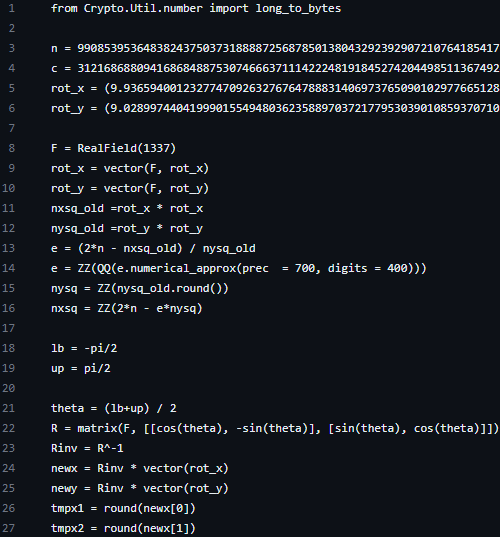
\includegraphics[width=0.6\linewidth]{Code1.png}
		     \label{fig:my_label}
		 \end{figure}
\end{frame}

\begin{frame}[c]
    \frametitle{Код}
		\begin{figure}
		     \centering
		     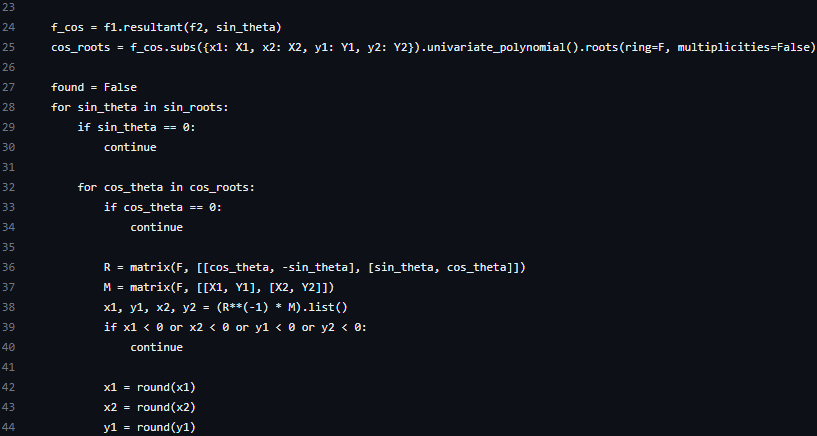
\includegraphics[width=0.65\linewidth]{Code2.png}
		     \label{fig:my_label}
		 \end{figure}
\end{frame}

\begin{frame}[c]
    \frametitle{Код}
		\begin{figure}
		     \centering
		     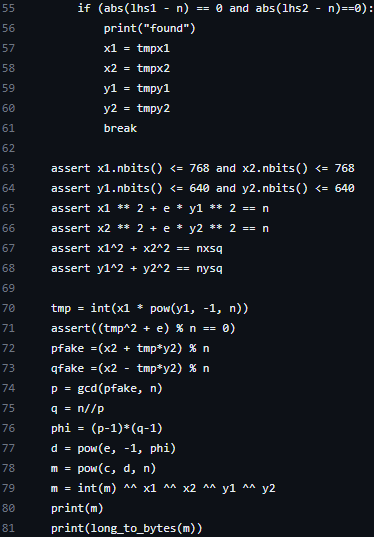
\includegraphics[width=0.46\linewidth]{Code3.png}
		     \label{fig:my_label}
		 \end{figure}
\end{frame}

\begin{frame}[c]
	\begin{block}{}
    \frametitle{Результат}
		 {В результате работы будет выведено значение флага:}
	\end{block}
    \begin{figure}
		     \centering
		     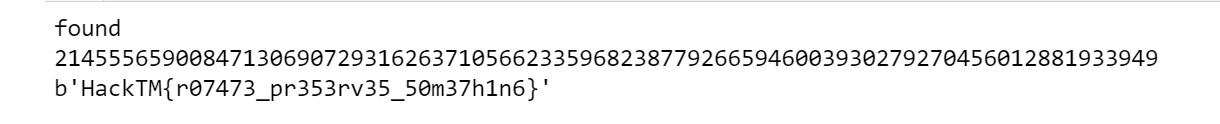
\includegraphics[width=1\linewidth]{Result.jpg}
		     \label{fig:my_label}
		 \end{figure}
\end{frame}

\begin{frame}[c]
    \frametitle{Ссылки}
	\begin{itemize}
		\item Код презентации и код задания: \href{https://github.com/KorkunoVl/Practice2023-Gervyatovich-Korshunov}{https://github.com/KorkunoVl/Practice2023-Gervyatovich-Korshunov}
	\end{itemize}	
\end{frame}

\end{document}